% P05 training-only smoke figure; not a model comparison on unseen data.
% data_sha256=48e1a384f932994448b539ec2f8e8de886893170c1f8f952359914470f815f3f
\documentclass[tikz,border=8pt]{standalone}
\usepackage{pgfplots}
\pgfplotsset{compat=1.18}
\usepgfplotslibrary{groupplots}
\ifdefined\pdfinfoomitdate\pdfinfoomitdate=1\fi
\ifdefined\pdfsuppressptexinfo\pdfsuppressptexinfo=-1\fi
\ifdefined\pdftrailerid\pdftrailerid{}\fi
\definecolor{p05Dzero}{HTML}{0072B2}
\definecolor{p05Done}{HTML}{E69F00}
\definecolor{p05Dtwo}{HTML}{009E73}
\definecolor{p05Dthree}{HTML}{CC79A7}
\begin{document}
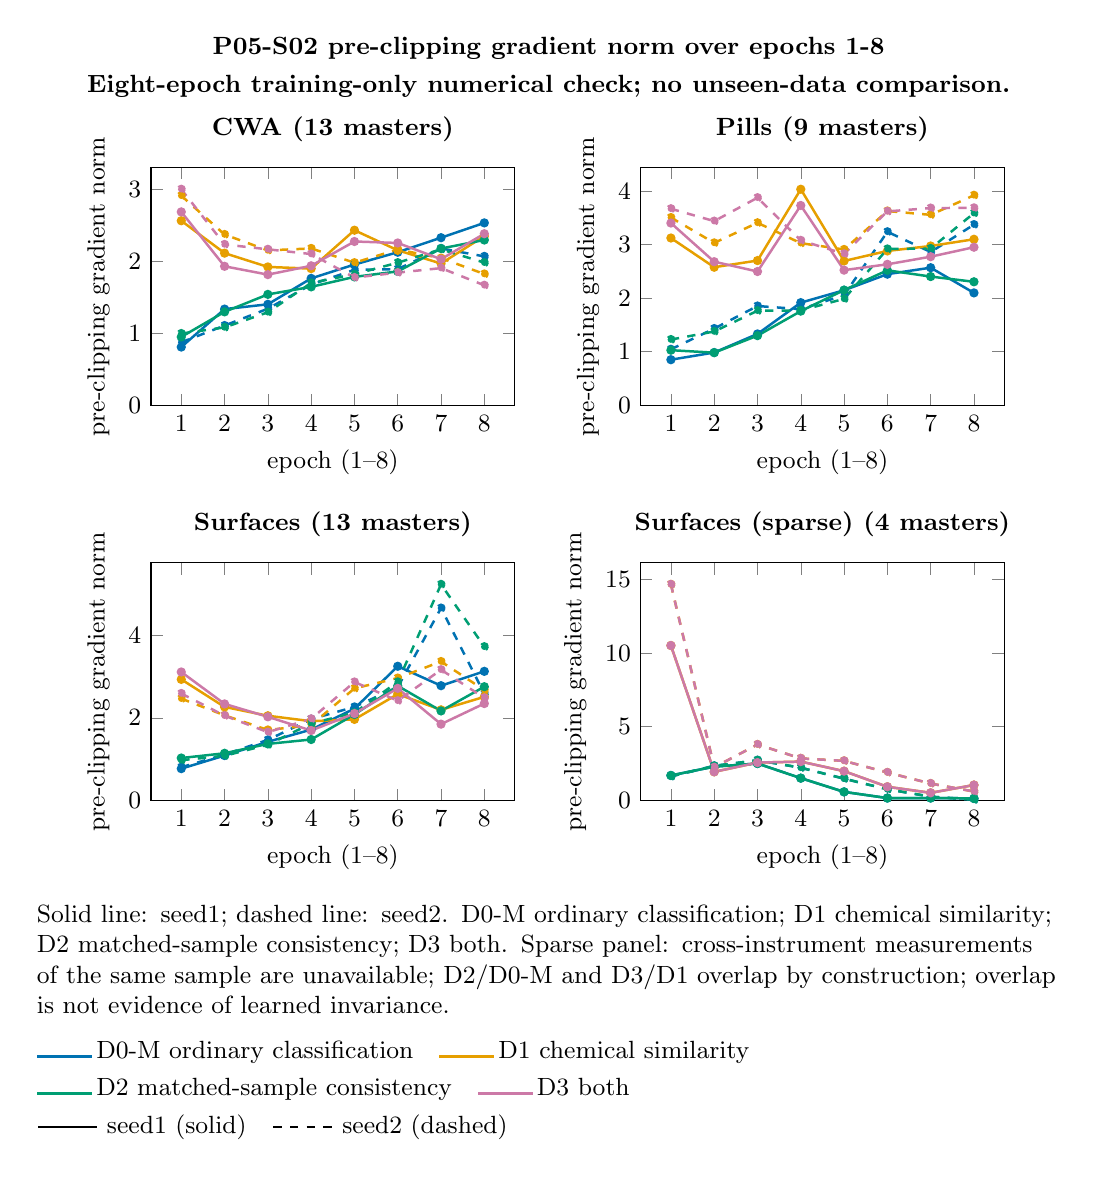
\begin{tikzpicture}
\begin{groupplot}[
  group style={group size=2 by 2, xlabels at=edge bottom, ylabels at=edge left, horizontal sep=1.6cm, vertical sep=2.0cm},
  width=6.2cm, height=4.6cm,
  every axis plot/.append style={line width=0.9pt},
  tick label style={font=\small, color=black},
  label style={font=\small, color=black},
  title style={font=\small\bfseries, color=black},
]
\nextgroupplot[title={CWA (13 masters)}, xlabel={epoch (1--8)}, ylabel={pre-clipping gradient norm}, xtick={1,...,8}, ymin=0]
\addplot[color=p05Dzero, solid, mark=*, mark size=1.2pt] coordinates {(1,0.80982846822419297) (2,1.3370225409370384) (3,1.4034348645610302) (4,1.7639478842732819) (5,1.9562985210293293) (6,2.1271648297242796) (7,2.3291955492122951) (8,2.534861545137864)};
\addplot[color=p05Dzero, dashed, mark=*, mark size=1.2pt] coordinates {(1,0.87630535447009716) (2,1.1083818717202407) (3,1.342603580671959) (4,1.678075148361974) (5,1.8825780062753319) (6,1.8924841245763639) (7,2.1796502198466801) (8,2.0691458683254211)};
\addplot[color=p05Done, solid, mark=*, mark size=1.2pt] coordinates {(1,2.5647732415147084) (2,2.1144955315765213) (3,1.9229430206782445) (4,1.8995196120943074) (5,2.4331550597033531) (6,2.1540209758295674) (7,1.9701145115637173) (8,2.351275200805063)};
\addplot[color=p05Done, dashed, mark=*, mark size=1.2pt] coordinates {(1,2.913119685977418) (2,2.3734625127922309) (3,2.1527436279654064) (4,2.1799909921648828) (5,1.9816363514708026) (6,2.1647856588474652) (7,2.0453267599355023) (8,1.8246179884074067)};
\addplot[color=p05Dtwo, solid, mark=*, mark size=1.2pt] coordinates {(1,0.9503787420695835) (2,1.2988698879476199) (3,1.5413302808071929) (4,1.645874279022103) (5,1.7848021850017004) (6,1.8607065765927666) (7,2.1785673506952796) (8,2.2969764956964283)};
\addplot[color=p05Dtwo, dashed, mark=*, mark size=1.2pt] coordinates {(1,0.99744285893575957) (2,1.0823287472040539) (3,1.2931552755324833) (4,1.7006069733705056) (5,1.8211836262558356) (6,1.9818755709123244) (7,2.1677664225930426) (8,1.9824448512971493)};
\addplot[color=p05Dthree, solid, mark=*, mark size=1.2pt] coordinates {(1,2.687839631690669) (2,1.9316482923906) (3,1.8162081154979359) (4,1.9389441256838562) (5,2.2765237323556557) (6,2.2559440428813327) (7,2.0302805893871199) (8,2.3844788366873098)};
\addplot[color=p05Dthree, dashed, mark=*, mark size=1.2pt] coordinates {(1,3.0023594354102094) (2,2.235256972074382) (3,2.1675371813647741) (4,2.1020861570919833) (5,1.7748784742024197) (6,1.8435520759813746) (7,1.9064817359273538) (8,1.6679561812240014)};
\nextgroupplot[title={Pills (9 masters)}, xlabel={epoch (1--8)}, ylabel={pre-clipping gradient norm}, xtick={1,...,8}, ymin=0]
\addplot[color=p05Dzero, solid, mark=*, mark size=1.2pt] coordinates {(1,0.85171427228548147) (2,0.98520015760622515) (3,1.3321173194378384) (4,1.916692812137839) (5,2.1473860189455816) (6,2.4482477319001852) (7,2.5687598324775571) (8,2.0982147898331056)};
\addplot[color=p05Dzero, dashed, mark=*, mark size=1.2pt] coordinates {(1,1.0453733993515673) (2,1.4325442810374311) (3,1.8535017895937331) (4,1.7943058989200484) (5,2.0569362179373076) (6,3.2389880040202144) (7,2.8613892508918601) (8,3.3727018779341118)};
\addplot[color=p05Done, solid, mark=*, mark size=1.2pt] coordinates {(1,3.1229452341406745) (2,2.5775343670202018) (3,2.7020313367760416) (4,4.0330791518759233) (5,2.6945501965173957) (6,2.8814269471841509) (7,2.9740788121313773) (8,3.0995194839380402)};
\addplot[color=p05Done, dashed, mark=*, mark size=1.2pt] coordinates {(1,3.5048302184417293) (2,3.0315822271761483) (3,3.4068073080304568) (4,3.0260399436514476) (5,2.9091670406716208) (6,3.6260833134463253) (7,3.5549665958454009) (8,3.9201481233574214)};
\addplot[color=p05Dtwo, solid, mark=*, mark size=1.2pt] coordinates {(1,1.0291703010766378) (2,0.98277222761659155) (3,1.3001952377225985) (4,1.7582248766512449) (5,2.1508772639945857) (6,2.5195989432166517) (7,2.4031707736696424) (8,2.3056809722140623)};
\addplot[color=p05Dtwo, dashed, mark=*, mark size=1.2pt] coordinates {(1,1.2273744541719844) (2,1.3777483954477445) (3,1.7655985974811128) (4,1.7711684868005269) (5,1.9871364938504144) (6,2.9178664052431538) (7,2.92685270423092) (8,3.5868713187464345)};
\addplot[color=p05Dthree, solid, mark=*, mark size=1.2pt] coordinates {(1,3.402308857359122) (2,2.6806922314569985) (3,2.4977591594274147) (4,3.7301915220932154) (5,2.5231973721495704) (6,2.6319870870638984) (7,2.7741330397882562) (8,2.9510558536437679)};
\addplot[color=p05Dthree, dashed, mark=*, mark size=1.2pt] coordinates {(1,3.6692318960858423) (2,3.437713332717975) (3,3.875230687569915) (4,3.0784700726091487) (5,2.8271549631850461) (6,3.6197551406137056) (7,3.6815188354977404) (8,3.6853296001596303)};
\nextgroupplot[title={Surfaces (13 masters)}, xlabel={epoch (1--8)}, ylabel={pre-clipping gradient norm}, xtick={1,...,8}, ymin=0]
\addplot[color=p05Dzero, solid, mark=*, mark size=1.2pt] coordinates {(1,0.77004519225062651) (2,1.0861975659179537) (3,1.4187838047057824) (4,1.7139880354465125) (5,2.2214476579828424) (6,3.2459750963667773) (7,2.7765713906886895) (8,3.1235978183118109)};
\addplot[color=p05Dzero, dashed, mark=*, mark size=1.2pt] coordinates {(1,0.80394307750113758) (2,1.1093279072996749) (3,1.4655822589982614) (4,1.9669284241036613) (5,2.262791057494927) (6,2.7427696226186695) (7,4.6537183653477872) (8,2.581438852911405)};
\addplot[color=p05Done, solid, mark=*, mark size=1.2pt] coordinates {(1,2.929157955671243) (2,2.2624452954619945) (3,2.0491827825797722) (4,1.9171658491901937) (5,1.961502646864604) (6,2.5722716929985521) (7,2.19257812782093) (8,2.5063958949786276)};
\addplot[color=p05Done, dashed, mark=*, mark size=1.2pt] coordinates {(1,2.4635436350988291) (2,2.0597319615746059) (3,1.7048379633658421) (4,1.8210270320254305) (5,2.7110325703712346) (6,2.9604985476118588) (7,3.3608841411145658) (8,2.6690427644550683)};
\addplot[color=p05Dtwo, solid, mark=*, mark size=1.2pt] coordinates {(1,1.0263516153274752) (2,1.1415970654498877) (3,1.3684216724324612) (4,1.4746605736097593) (5,2.080546758939199) (6,2.7720640096946041) (7,2.1659938587587524) (8,2.7522152486071154)};
\addplot[color=p05Dtwo, dashed, mark=*, mark size=1.2pt] coordinates {(1,0.97396043988202852) (2,1.0800908376131428) (3,1.3484535976405843) (4,1.8606433454315034) (5,2.1239938393015003) (6,2.8675702929072577) (7,5.2265416398221776) (8,3.7194597909925715)};
\addplot[color=p05Dthree, solid, mark=*, mark size=1.2pt] coordinates {(1,3.1078098882820067) (2,2.335938898445697) (3,2.023238666639168) (4,1.692027106082447) (5,2.1027745002142071) (6,2.7114368302780347) (7,1.8462708766076652) (8,2.3449005620882275)};
\addplot[color=p05Dthree, dashed, mark=*, mark size=1.2pt] coordinates {(1,2.5872458680542643) (2,2.0513805734457389) (3,1.6518730708128166) (4,1.9744111393260373) (5,2.8659217698336601) (6,2.4123439511736389) (7,3.1627104974471099) (8,2.4826338873060791)};
\nextgroupplot[title={Surfaces (sparse) (4 masters)}, xlabel={epoch (1--8)}, ylabel={pre-clipping gradient norm}, xtick={1,...,8}, ymin=0]
\addplot[color=p05Dzero, solid, mark=*, mark size=1.2pt] coordinates {(1,1.6976951085917549) (2,2.2948388419027639) (3,2.5055937680660518) (4,1.5146401409315686) (5,0.58188189390001122) (6,0.16267684429005355) (7,0.16638862790224113) (8,0.14170075579168984)};
\addplot[color=p05Dzero, dashed, mark=*, mark size=1.2pt] coordinates {(1,1.6294823988362395) (2,2.3458990187978204) (3,2.7276355979085043) (4,2.2217125107685396) (5,1.4770364378749017) (6,0.75853425674358532) (7,0.25932477180435382) (8,0.048650858481379559)};
\addplot[color=p05Done, solid, mark=*, mark size=1.2pt] coordinates {(1,10.510583427436275) (2,1.9420605099155444) (3,2.5690138708825501) (4,2.6360616112406858) (5,1.9887446048367015) (6,0.92815308739898705) (7,0.51850515920124318) (8,1.0470315012180962)};
\addplot[color=p05Done, dashed, mark=*, mark size=1.2pt] coordinates {(1,14.654289577181025) (2,2.2513067609058042) (3,3.7940011810847212) (4,2.8539029625600989) (5,2.6844034473555758) (6,1.8975988055368913) (7,1.1489303229871211) (8,0.60681576961342054)};
\addplot[color=p05Dtwo, solid, mark=*, mark size=1.2pt] coordinates {(1,1.6976951085917549) (2,2.2948388419027639) (3,2.5055937680660518) (4,1.5146401409315686) (5,0.58188189390001122) (6,0.16267684429005355) (7,0.16638862790224113) (8,0.14170075579168984)};
\addplot[color=p05Dtwo, dashed, mark=*, mark size=1.2pt] coordinates {(1,1.6294823988362395) (2,2.3458990187978204) (3,2.7276355979085043) (4,2.2217125107685396) (5,1.4770364378749017) (6,0.75853425674358532) (7,0.25932477180435382) (8,0.048650858481379559)};
\addplot[color=p05Dthree, solid, mark=*, mark size=1.2pt] coordinates {(1,10.510583427436275) (2,1.9420605099155444) (3,2.5690138708825501) (4,2.6360616112406858) (5,1.9887446048367015) (6,0.92815308739898705) (7,0.51850515920124318) (8,1.0470315012180962)};
\addplot[color=p05Dthree, dashed, mark=*, mark size=1.2pt] coordinates {(1,14.654289577181025) (2,2.2513067609058042) (3,3.7940011810847212) (4,2.8539029625600989) (5,2.6844034473555758) (6,1.8975988055368913) (7,1.1489303229871211) (8,0.60681576961342054)};
\end{groupplot}
\node[anchor=south, font=\bfseries\small, color=black, align=center, text width=13cm] at (current bounding box.north) {P05-S02 pre-clipping gradient norm over epochs 1-8\\[1mm]Eight-epoch training-only numerical check; no unseen-data comparison.};
\node[anchor=north, font=\small, color=black, align=left, text width=13cm] (p05caption) at ([yshift=-2mm]current bounding box.south) {Solid line: seed1; dashed line: seed2. D0-M ordinary classification; D1 chemical similarity; D2 matched-sample consistency; D3 both. Sparse panel: cross-instrument measurements of the same sample are unavailable; D2/D0-M and D3/D1 overlap by construction; overlap is not evidence of learned invariance.};
\node[anchor=north west, font=\small, color=black, align=left, text width=13cm] at ([yshift=-1mm]p05caption.south west) {\textcolor{p05Dzero}{\rule{7mm}{1.2pt}}\,D0-M ordinary classification\quad \textcolor{p05Done}{\rule{7mm}{1.2pt}}\,D1 chemical similarity\\[0.8mm]\textcolor{p05Dtwo}{\rule{7mm}{1.2pt}}\,D2 matched-sample consistency\quad \textcolor{p05Dthree}{\rule{7mm}{1.2pt}}\,D3 both\\[1mm]\tikz[baseline=-0.6ex]\draw[black,solid,line width=0.9pt](0,0)--(0.75,0);\ seed1 (solid)\quad \tikz[baseline=-0.6ex]\draw[black,dashed,line width=0.9pt](0,0)--(0.75,0);\ seed2 (dashed)};
\end{tikzpicture}
\end{document}
